\chapter{Hauptkapitel\#1}

Dieses Kapitel konkretisiert die bereits genannten Problematiken, schildert und vergleicht mögliche Umsetzungsvarianten, um diese zu vergleichen und daraus eine Auswahl zu treffen.
Hier werden regelmäßig die Grundlagen referenziert.


\section{weitere Beispiele}

\begin{table}[ht]
\centering
    \begin{tabular}{l r | r}
        \hline\hline
        \thead{Tabelle}
        &
        \thead{\# Einträge}
        &
        \thead{Proz. Anteil der\\ursprünglichen Einträge} \\ [0.5ex] 
        % \thead erlaubt Zeilenumbruch in header
        % [0.5ex] = Abstand zur nächsten Zeile
        \hline
        Face Position Orientation   & $\sim$ 67.847.000 (73.3 \%) &  100.0 \%\\
        Face Demographics           & $\sim$ 24.377.000 (26.3 \%) &   36.0 \%\\
        Image Details               &    $\sim$ 161.000 ( 0.2 \%) &    0.2 \%\\
        Face Details                &    $\sim$ 144.000 ( 0.2 \%) &    0.2 \%\\
        \hline
        \textbf{Gesamt}             &        92.528.750 (100 \%)  &  \\ [1ex]
        \hline\hline
    \end{tabular}
\caption{Verteilung der Einträge auf die gruppierten Tabellen}
\label{tab:verteilung}
\end{table}

\clearpage

\begin{wrapfigure}{l}{0.5\linewidth}
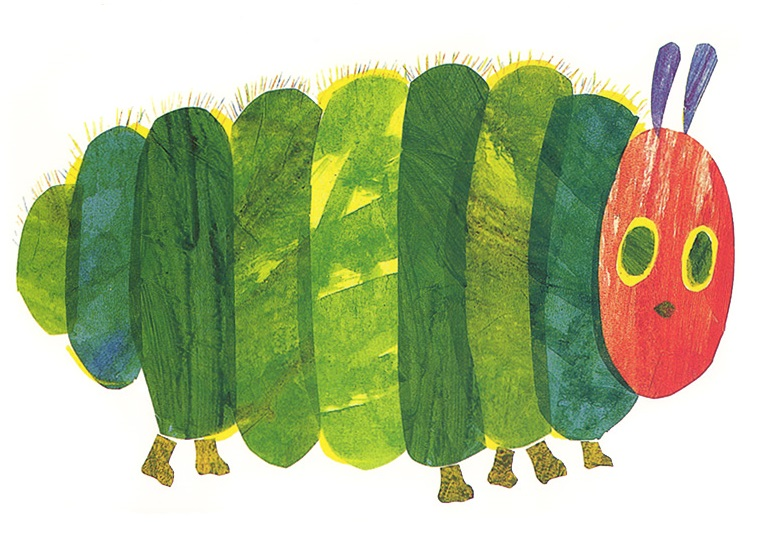
\includegraphics[width=\linewidth]{bilder/caterpillar.jpg}
\caption[Caterpillar]{Caterpillar\cite{caterpillar}}
\label{fig:caterpillar}
\end{wrapfigure}

Im Gegensatz dazu sind die Tabellen der Bilder, Gesichter und Annotationen sehr dicht zusammenhängend.
Bei beinahe allen Anfragen der Annotationen werden zugleich die Gesichter und Bilder benötigt.
Somit werden für diese Fälle die drei Tabellen der ursprünglichen Datenbank zu einer Collection kombiniert, bzw. verkettet, sodass nur eine Anfrage benötigt wird. 
Denn wären diese getrennt, würden drei Anfragen benötigt werden, wobei auf Grund der 1:n Beziehungen für jede Annotation und wiederum jedes Gesicht ein lookup benötigt wäre.
Dies würde dazu führen, dass es bei Millionen von Einträgen zu enormen Performance Verlusten kommt.

\begin{table}[hb]
\scriptsize
\begin{minipage}{0.49\linewidth}
\centering
\begin{tabular}{||c | r | r | r |} 
    \hline
    \textbf{Nr.} & \textbf{\# Ergeb.} & \textbf{PostgreSQL} & \textbf{MongoDB} \\ [0.5ex]
    \hline\hline
    \multirow{3}{*}{1.1} & \multirow{3}{*}{4.678} 
      & 0,9548 s & 0,3056 s \\
    & & 0,8997 s & 0,1290 s \\
    & & 0,9101 s & 0,1213 s \\
    \hline
    \multirow{3}{*}{1.2} & \multirow{3}{*}{4.678} 
      & 1,1088 s & -- \\
    & & 1,2218 s & -- \\
    & & 1,2137 s & -- \\
    \hline
    \multirow{3}{*}{1.3} & \multirow{3}{*}{4.678} 
      & 0,0403 s & -- \\
    & & 0,0412 s & -- \\
    & & 0,0401 s & -- \\
    \hline
    \multirow{3}{*}{2} & \multirow{3}{*}{4.678} 
      & 0,9498 s & 0,1466 s \\
    & & 0,9729 s & 0,1083 s \\
    & & 0,9071 s & 0,1066 s \\
    \hline
    \multirow{3}{*}{3} & \multirow{3}{*}{10.043} 
      & 0,2779 s & 0,3600 s \\
    & & 0,3079 s & 0,2429 s \\
    & & 0,2992 s & 0,2498 s \\
    \hline
    \multirow{3}{*}{4} & \multirow{3}{*}{2} 
      & 0,0018 s & 0,0727 s \\
    & & 0,0009 s & 0,0138 s \\
    & & 0,0009 s & 0,0070 s \\
    \hline
    \multirow{3}{*}{5} & \multirow{3}{*}{253.755}
      & 3,5117 s & 126,0782 s \\
    & & 3,4656 s & 106,1470 s \\
    & & 3,3282 s & 107,9439 s \\
    \hline
\end{tabular}
\end{minipage}
%
\begin{minipage}{0.49\linewidth}
\centering
\begin{tabular}{|c | r | r | r ||} 
    \hline
    \textbf{Nr.} & \textbf{\# Ergeb.} & \textbf{PostgreSQL} & \textbf{MongoDB} \\ [0.5ex] 
    \hline\hline 
    \multirow{3}{*}{6} & \multirow{3}{*}{5.141}
      & 2,1497 s & 12,1915 s \\
    & & 1,8485 s & 11,6134 s \\
    & & 1,7347 s & 11,2647 s \\
    \hline
    \multirow{3}{*}{7} & \multirow{3}{*}{694.907} 
      & 6,3388 s & 23,2439 s \\
    & & 6,6917 s & 22,4676 s \\
    & & 6,6002 s & 22,9043 s \\
    \hline
    \multirow{3}{*}{8} & \multirow{3}{*}{0} 
      & 0,0018 s & 0,0011 s \\
    & & 0,0008 s & 0,0009 s \\
    & & 0,0008 s & 0,0008 s \\
    \hline
    \multirow{3}{*}{9.1} & \multirow{3}{*}{1.635.965} 
      & 27,0328 s & 68,7589 s \\
    & & 28,4229 s & 58,9914 s \\
    & & 27,9176 s & 64,8253 s \\
    \hline
    \multirow{3}{*}{9.2} & \multirow{3}{*}{1.635.965} 
      & 12,2981 s & 73,4722 s \\
    & & 11,5675 s & 63,1674 s \\
    & & 11,4067 s & 68,5112 s \\
    \hline
    \multirow{3}{*}{10.1} & \multirow{3}{*}{14.222.062} 
      & 113,2476 s & 373,5514 s \\
    & & 107,6503 s & 370,8531 s \\
    & & 112,4459 s & 373,4111 s \\
    \hline
    \multirow{3}{*}{10.2} & \multirow{3}{*}{14.222.062} 
      & 143,6760 s & -- \\
    & & 141,0328 s & -- \\
    & & 142,5101 s & -- \\
    \hline
\end{tabular}
\end{minipage}
\caption{Beispieltabelle eines Benchmarks}
\label{tab:benchmark_results}
\end{table}
